%%%%%%%%%%%%%%%%%%%%%%%%%%%%%%%%%%%%%%%%%%%%%%%%%%%%%%%%%%%%%%%%%%
%%%%%%%% ICML 2017 EXAMPLE LATEX SUBMISSION FILE %%%%%%%%%%%%%%%%%
%%%%%%%%%%%%%%%%%%%%%%%%%%%%%%%%%%%%%%%%%%%%%%%%%%%%%%%%%%%%%%%%%%

% Use the following line _only_ if you're still using LaTeX 2.09.
%\documentstyle[icml2017,epsf,natbib]{article}
% If you rely on Latex2e packages, like most moden people use this:
\documentclass{article}

% use Times
\usepackage{times}
% For figures
\usepackage{graphicx} % more modern
%\usepackage{epsfig} % less modern
\usepackage{subfigure} 

% For citations
\usepackage{natbib}

% For algorithms
\usepackage{algorithm}
\usepackage{algorithmic}

% As of 2011, we use the hyperref package to produce hyperlinks in the
% resulting PDF.  If this breaks your system, please commend out the
% following usepackage line and replace \usepackage{icml2017} with
% \usepackage[nohyperref]{icml2017} above.
\usepackage{hyperref}

% Packages hyperref and algorithmic misbehave sometimes.  We can fix
% this with the following command.
\newcommand{\theHalgorithm}{\arabic{algorithm}}

% Employ the following version of the ``usepackage'' statement for
% submitting the draft version of the paper for review.  This will set
% the note in the first column to ``Under review.  Do not distribute.''
\usepackage{icml2017} 
%\usepackage[accepted]{icml2017}

% Added by Chandan
\usepackage{tabulary} % for tables
\usepackage{amsmath}
\newcommand{\scell}[2][c]{\begin{tabular}[#1]{@{}c@{}}#2\end{tabular}}
\usepackage{placeins}
\usepackage{float}
% The \icmltitle you define below is probably too long as a header.
% Therefore, a short form for the running title is supplied here:
\icmltitlerunning{A Weighted-$\ell_1$, Multi-task Graphical Model }

\begin{document} 

\twocolumn[
\icmltitle{A Weighted-$\mathbf{\ell_1}$, Multi-task Graphical Model \\
	with Applications to Heterogenous Brain Connectivity}

% It is OKAY to include author information, even for blind
% submissions: the style file will automatically remove it for you
% unless you've provided the [accepted] option to the icml2017
% package.

% list of affiliations. the first argument should be a (short)
% identifier you will use later to specify author affiliations
% Academic affiliations should list Department, University, City, Region, Country
% Industry affiliations should list Company, City, Region, Country

% you can specify symbols, otherwise they are numbered in order
% ideally, you should not use this facility. affiliations will be numbered
% in order of appearance and this is the preferred way.
\icmlsetsymbol{equal}{*}

\begin{icmlauthorlist}
\icmlauthor{Chandan Singh}{uva}
\icmlauthor{Beilun Wang}{uva}
\icmlauthor{Yanjun Qi}{uva}
\end{icmlauthorlist}

\icmlaffiliation{uva}{University of Virginia, Charlottesville, Virginia, USA}
\icmlcorrespondingauthor{Yanjun Qi}{yq2h@virginia.edu}

% You may provide any keywords that you 
% find helpful for describing your paper; these are used to populate 
% the "keywords" metadata in the PDF but will not be shown in the document
\icmlkeywords{weighted-l1, multi-task, joint, functional connectivity}

\vskip 0.3in
]

% this must go after the closing bracket ] following \twocolumn[ ...

% This command actually creates the footnote in the first column
% listing the affiliations and the copyright notice.
% The command takes one argument, which is text to display at the start of the footnote.
% The \icmlEqualContribution command is standard text for equal contribution.
% Remove it (just {}) if you do not need this facility.

\printAffiliationsAndNotice{}  % leave blank if no need to mention equal contribution
%\printAffiliationsAndNotice{\icmlEqualContribution} % otherwise use the standard text.

\begin{abstract} 
	This work introduces a novel, weighted-$\ell_1$, multi-task graphical model (WELM) for determining functional connectivity. The weighted-$\ell_1$ norm induces sparsity while simultaneously imposing a prior that is specified on each edge. Here, applications to brain data with a spatial prior show state-of-the art connectivity determination.
\end{abstract} 

\section{Introduction}
\label{sec:introduction}
\subsection{Connectivity} Many problems can be formulated as finding an undirected graph over different regions representing conditional correlations in activity between the regions. For example, there has been great interest in mapping the interactions between brain regions, a field known as functional connectomics \cite{seung2011neuroscience, smith2013functional}. The resulting graphs, or connectomes, have many potential uses such as understanding the differences between those with typically developing brains and those with clinical disorders \cite{uddin2013salience,milham2012adhd}. With advancements in functional Magnetic Resonance Imaging (fMRI), connectomes are increasingly detailed, creating a need for novel algorithms to interpret this data.

Mathematically, determining functional connectivity amounts to first calculating a covariance matrix ($\Sigma$) from the data and then estimating the connectivity graph with the precision matrix ($\Omega=\Sigma^{-1}$). Zeros in $\Omega$ correspond to conditionally independent nodes, while non-zero values represent conditional edges \cite{lauritzen1996graphical}. Accurately estimating the precision matrix is computationally difficult because of problems with high-order correlations between feature variables \cite{fan2013statistical}. Thus, this problem is well-suited to graphical models, which are able to pick out conditional correlations from high-order data \cite{koller2007graphical}. Specifically, a sparse Gaussian Graphical Model can be utilized to reliably estimate $\Omega$ by limiting the number of nonzero connections in the precision matrix via $\ell_1$ penalization \cite{friedman2008sparse,banerjee2008model}.

\subsection{Weighted-$\ell_1$, Multi-task Learning}
In several connectivity problems, there is prior knowledge regarding which edges are most likely to be zero. Thus, weights can be associated with edges to penalize their inclusion in the estimated connectivity graph. For fMRI recordings, these weights can be the spatial distances between connections, since the brain favors short connections due to space and energy constraints \cite{watts1998collective}. For problems with few data samples, this can improve robust connectivity estimation.

A common problem in applications is to estimate connectivity for more than one group, \textit{e.g.} a disease group and a control group. In this problem, referred to as multi-task learning, modeling a shared set of parameters between groups improves the overall estimation of the parameters. A variety of recent multi-task graphical models exist, but they have seen limited application to estimating functional connectivity in the brain. Here, several state-of-the-art multi-task models are compared on a real-world dataset. A depiction of weighted-$\ell_1$, multi-task learning is shown in Figure~\ref{fig:intro}.

\begin{figure}[H]
	\centering
	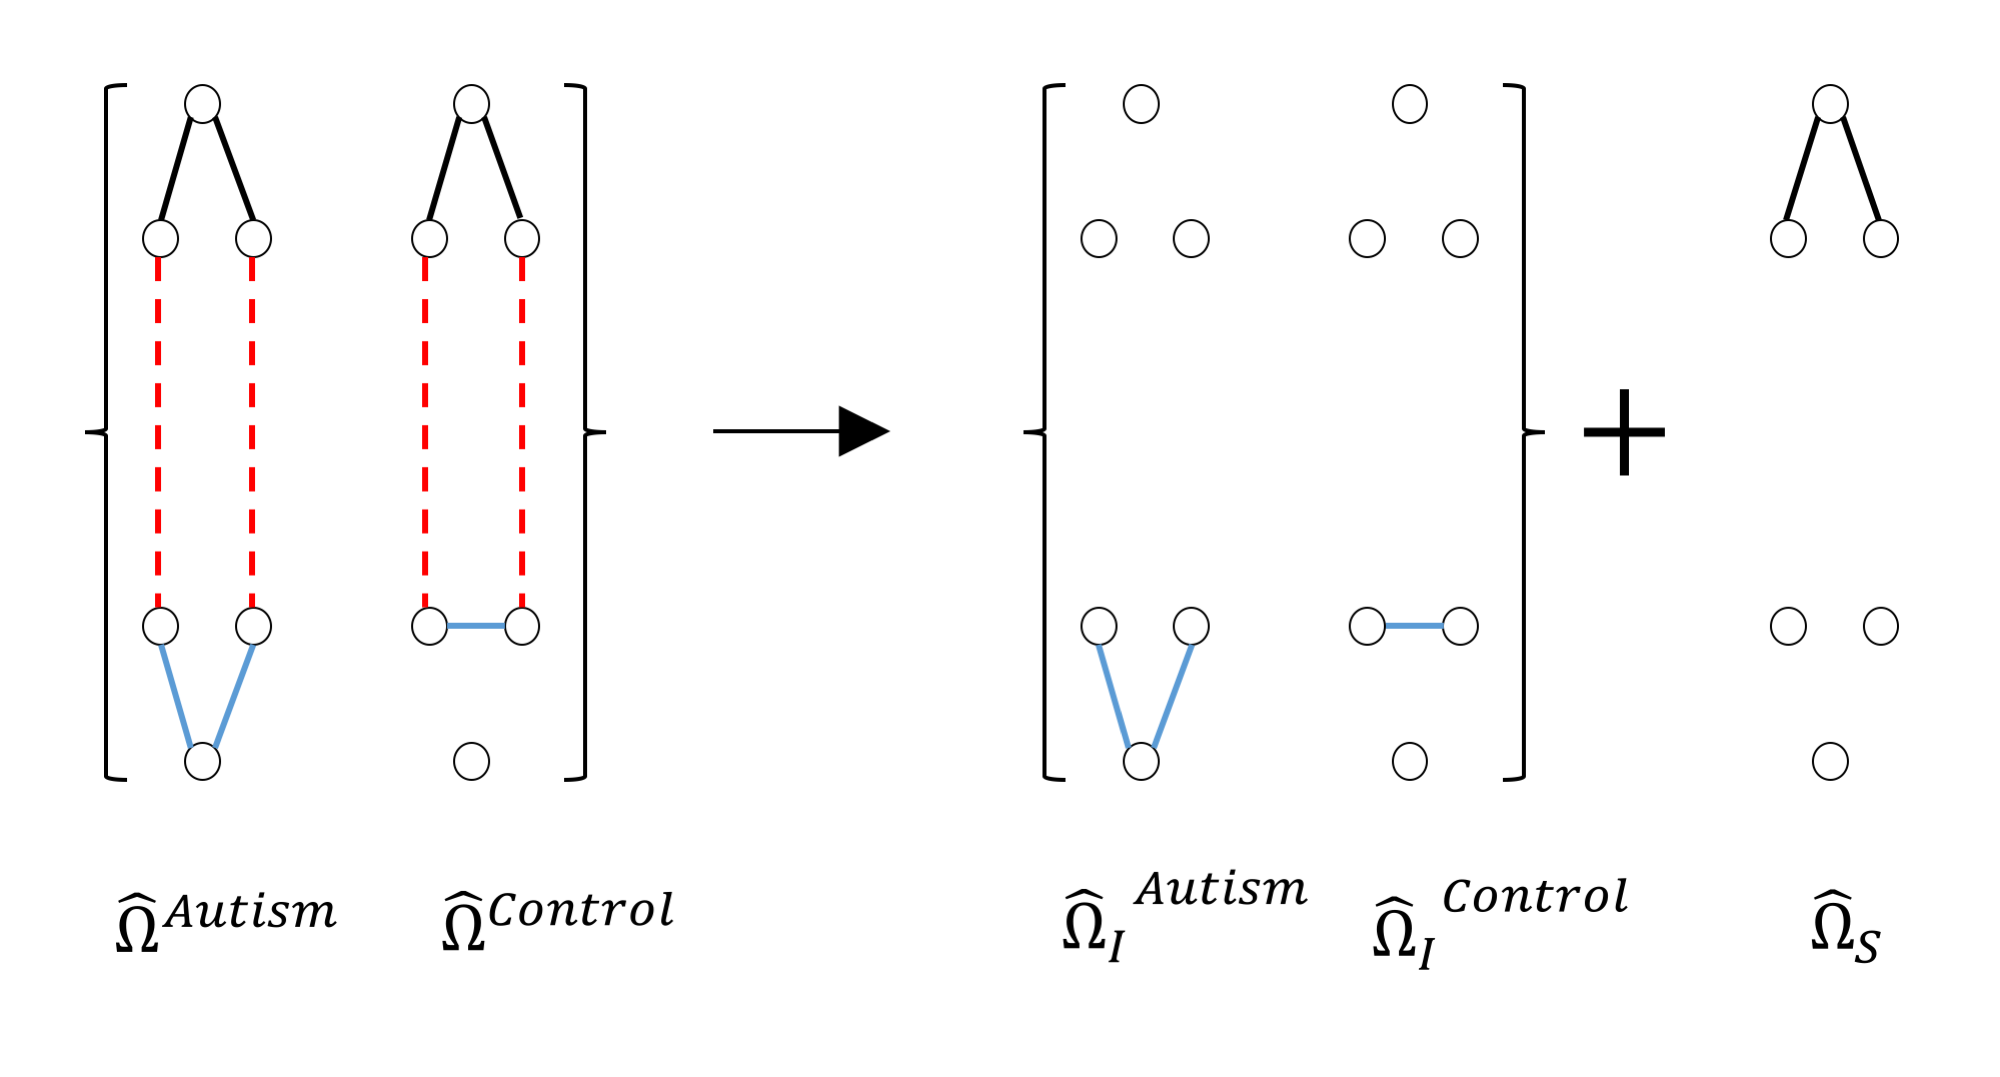
\includegraphics[width=\columnwidth]{../../plots/intro/intro.png}
	\caption{Demonstration of utility of weighted-$\ell_1$, multi-task learning. Here, long-distance edges (red dashed lines) are penalized and thus not learned. Black edges are shared between groups and are learned as shared parameters. Blue edges are task-specific and are learned in individual groups.}
	\label{fig:intro}
\end{figure}

\subsection{Novel Contributions}
This study's main contribution is the novel formulation of a weighted-$\ell_1$, multi-task graphical model (WELM) which can be applied to a variety of different datasets. Additionally, this study examines a particular resting-state fMRI dataset which serves to compare and validate several recent multi-task learning models. Classification by the novel model here outperforms the state-of-the-art on this dataset.

The organization of the paper is as follows. Section~\ref{sec:model} details the novel model, Section~\ref{previous_work} reviews previous work, Section~\ref{experiments} shows experiments validating WELM, and Section~\ref{conclusions} explains our conclusions.

\section{WELM: A Weighted-$\ell_1$ , Multi-task Model}
\label{sec:model}
\subsection{Notation}
In the work that follows, $k$ is the number of groups, $||\cdot ||_1$ represents the $\ell_1$ norm, $||\cdot ||_\infty$ represents the $\ell_\infty$ norm, $W$ is a prior matrix of positive weights, $\Sigma$ is the covariance matrix, and we define the dot product ($\cdot$) between two matrices to be their elementwise dot product. Furthermore, we define $\Omega^{(i)}$ as the precision matrix for a group $i$ and model it as two parts:
\begin{equation}
\label{eq:omega_i}
\Omega^{(i)} = \Omega_I^{(i)} + \Omega_S
\end{equation}
where $\Omega_I^{(i)}$ is the individual precision matrix for group $i$ and $\Omega_S$ is the shared precision matrix between groups.

\subsection{Formulation}
The model starts with a simple $\ell_1$ penalty, which yields a precision matrix for each group.
\begin{equation}
\label{eq:model_simule}
\begin{split}
\hat{\Omega}^{(1)},...,\hat{\Omega}^{(k)} = \underset{i}{\sum} \underset{\Omega^{(i)}}{\text{argmin}} || \Omega^{(i)} ||_1\\
\text{Subject to: } ||\Sigma^{(i)} (\Omega^{(i)} - I)|| _{\infty} \leq \lambda, i=1,...,k.
\end{split}
\end{equation}
Next, explicitly modeling the shared and individual parameters of each precision matrix separately yields the formulation of SIMULE \cite{wang2016constrained}, an effective multi-task model.
\begin{equation}
\label{eq:model_simule}
\begin{split}
\hat{\Omega}^{(1)}_I,...,\hat{\Omega}^{(k)}_I,\hat{\Omega}_S = \underset{i}{\sum} \underset{\Omega_I^{(i)},\Omega_S}{\text{argmin}} || \Omega_I^{(i)} ||_1  + \epsilon k|| \Omega_S  ||_1 \\
\text{Subject to: } ||\Sigma^{(i)} (\Omega_I^{(i)}+\Omega_S) - I|| _{\infty} \leq \lambda, i=1,...,k.
\end{split}
\end{equation}
Finally, the $\ell_1$ norm of each precision matrix is weighted by the prior matrix $W$, resulting in the novel formulation of WELM:
\begin{equation}
\label{eq:model_formulation}
\begin{split}
\hat{\Omega}^{(1)}_I,...,\hat{\Omega}^{(k)}_I,\hat{\Omega}_S = \underset{i}{\sum} \underset{\Omega_I^{(i)},\Omega_S}{\text{argmin}} || W \cdot \Omega_I^{(i)} ||_1  + \epsilon k|| W \cdot \Omega_S  ||_1 \\
\text{Subject to: } ||\Sigma^{(i)} (\Omega_I^{(i)}+\Omega_S) - I|| _{\infty} \leq \lambda, i=1,...,k.
\end{split}
\end{equation}

WELM has a flexible prior ($W$) and two hyperparameters ($\lambda,\text{and }\epsilon$) that allow it to be incredibly flexible. Using a different $W$ can enforce a different prior or change how strongly a prior is enforced. Next, changing the hyperparameter $\lambda$ controls the total sparsity of the resulting precision matrices. Finally, changing the hyperparameter $\epsilon$ allows for controlling how strongly the group penalty is imposed, $e.g.$ the relative sparsities between the shared parameters and the individual parameters.

\subsection{Model Benefits}
The model poses numerous benefits in addition to its ability to generate a sparse, prior-enforced, multi-task graph. The model can support more than just Gaussian data. If the kendall correlation matrix is used in place of the covariance matrix, WELM can learn nonparanormal Gaussian data (referred to as NWELM). Next, the formulation can be solved in parallel. The model's convergence is evident from proofs of the similar formulation of SIMULE \cite{wang2016constrained} combined with the fact that the positive weights in $W$ yield a convex norm.

\section{Previous work}
\label{previous_work}
\begin{table*}[ht]
	\caption{Summary of relevant previous work.}
	\label{tab:baselines}
	\vskip 0.15in
	\begin{center}
		\begin{small}
			\begin{sc}
				\begin{tabular}{lcccc}
					\hline
					\abovespace\belowspace
					Method & \scell{Conditional\\Independence} & \scell{Multi-\\task} & \scell[]{Column-wise\\Parallelizable} & \scell[]{Imposes\\ Prior}\\
					\hline
					\abovespace
					WELM & $\surd$ & $\surd$ & $\surd$ & $\surd$ \\
					CLIME & $\surd$ & $\surd$ & $\times$ & $\times$ \\
					GLASSO & $\surd$ & $\surd$ & $\times$ & $\times$ \\
					JGL & $\surd$ & $\surd$ & $\times$ & $\times$ \\
					DPM & $\surd$ & $\surd$ & $\times$ & $\times$ \\
					Spatial Regularization & $\times$ & $\times$ & $\times$ & $\surd$ \\
					sGGGM & $\surd$ & $\surd$ & $\times$ & $\times$ \\
					MNS & $\surd$ & $\surd$ & $\times$ & $\times$ \\
					SIMONE & $\surd$ & $\surd$ & $\times$ & $\times$ \\
					\belowspace
					SIMULE & $\surd$ & $\surd$ & $\surd$ & $\times$ \\
					\hline
				\end{tabular}
			\end{sc}
		\end{small}
	\end{center}
	\vskip -0.1in
\end{table*}

\subsection{Weighted-$\ell_1$ Models}
\label{weighted_penalization}

$\ell_1$ norms effectively induce sparsity in graphical models \cite{friedman2008sparse}. Importantly, by weighting the $\ell_1$ norm with a prior, the norm can induce sparsity while simultaneously penalizing the selection of certain edges. This differs from the reweighted-$\ell_1$ minimization commonly used in compressed sensing, which typically equips a general linear model to robustly impose sparsity with very few samples \cite{candes2008enhancing}. Some recent studies use a weighted-$\ell_1$ norm to enforce a prior while maintaining sparsity. For example, one previous model uses reweighted-$\ell_1$ norms to maintain sparsity while reducing penalties on nodes high degree, thus encouraging the appearance of ``hub" nodes with high degree \cite{liu2011learning}. Another study uses weighted-$\ell_1$ optimization for gene network estimation \cite{shimamura2007weighted}. However, none of these weighted-$\ell_1$ studies extends to brain connectivity or the multi-task setting.

\subsection{Brain Connectivity Priors}
WELM here requires choosing and enforcing a prior for functional brain connectivity. Spatial distance is a strong candidate, as spatial constraints are sufficient to capture a significant amount of connectivity via generative modeling \cite{vertes2012simple}. Previous studies have utilized spatial penalization, but use it for smoothing rather than feature selection \cite{baldassano2012voxel,ng2011generalized,grosenick2011family}. That is, weights on edges are fed into an $\ell_2$ norm to induce spatial smoothness.

\subsection{Multi-task Models}
\label{multi-task_models}
Two recent studies apply multi-task learning to brain connectivity determination. Mixed Neighborhood Selection \cite{monti2015learning} is an algorithm designed for learning population and subject-specific connectivity in brain networks, but isn't meant for discerning between two large classes, as is done here. Another recent study applies sparsity in a multi-task setting to functional connectivity determination \cite{ng2013novel}.

Here, comparisons are made to the two most-cited graphical models for multi-task learning JGL \cite{danaher2014joint} and SIMONE \cite{chiquet2011inferring}, and two more recent models with formulations closer to the one here: CLIME \cite{cai2011constrained} and SIMULE \cite{wang2016constrained}. As a baseline, all models are compared against the extremely popular graphical lasso (GLASSO) \cite{friedman2008sparse}. A final comparison is made to DPM, a model that directly predicts the differences between two classes \cite{zhao2014direct}. All studies are summarized in Table~\ref{tab:baselines}.
%\FloatBarrier
\section{Experiments}
\label{experiments}
\subsection{Data}
The data examined here comes from the Autism Brain Imaging Data Exchange (ABIDE) \cite{di2014autism}, a publicly available resting-state fMRI dataset. This includes fMRI recordings acquired from several international sites. Data was retrieved from the Preprocessed Connectomes Project \cite{craddock2014preprocessed}, where preprocessing was performed using the Configurable Pipeline for the Analysis of Connectomes (CPAC) \cite{craddock2013towards} with no global signal correction and no band-pass filtering. After successful preprocessing with this pipeline, 871 individuals remain. Signals for the 160 ROIs in the Dosenbach Atlas \cite{dosenbach2010prediction} are examined.

To weight the $\ell_1$ norm, two separate priors were derived from the Dosenbach atlas \cite{dosenbach2010prediction}. The first gave each ROI one of forty well-known, anatomic labels (e.g. ``basal ganglia", ``thalamus", ``lateral cerebellum"). Weights were then given a low constant value if two ROIs had the same label, and a high constant value if two ROIs had different labels. The second prior was the spatial distance, in MNI space, between the ROIs. The graphical method here is used to generate connectomes at varying levels of sparsity by sweeping over the regularization parameter $\lambda$, and the resulting average edge length is plotted against the total number of edges in each graph. When the weight matrix is raised to a power, thus increasing the spread of the distances (all distances are greater than 1), the prior is enforced more strongly. Experimental designed summarized in Table~\ref{tab:experimental_design}.

\begin{table*}[ht]
	\caption{Experimental design summary.}
	\label{tab:experimental_design}
	\vskip 0.15in
	\begin{center}
		\begin{small}
			\begin{sc}
				\begin{tabular}{lcc}
					\hline\\
					\multicolumn{3}{c}{Data}\\
					\hline
					\abovespace
					Number Autism Subjects & 468\\
					Number Control Subjects & 403\\
					Total Subjects &  871\\
					Preprocessing & CPAC & \scell[]{No global signal correction\\/ band-pass filtering}\\
					\belowspace
					ROIs examined & 160 & Dosenbach Atlas\\
					\hline
					
					\abovespace\belowspace
					Prior Name & Prior Description & Edge Weight\\
					\hline
					Distance & MNI distance between edges & Continuous value\\
					$\text{Distance}^2$ & MNI distance between edges squared & Continuous value\\
					Anatomical1 & \scell[]{One of 40 labels\\(e.g. ``basal ganglia", ``thalamus") }& 
					$\begin{cases}
					0.1& \text{if same label}\\
					0.9 & \text{otherwise}
					\end{cases}$\\
					\belowspace
					Anatomical2 & \scell[]{One of 40 labels\\(e.g. ``basal ganglia", ``thalamus") }& 
					$\begin{cases}
						0.2& \text{if same label}\\
						0.8 & \text{otherwise}
					\end{cases}$\\
					\hline
				\end{tabular}
			\end{sc}
		\end{small}
	\end{center}
	\vskip -0.1in
\end{table*}
\FloatBarrier

\subsection{Model Performance}
The most often-used metric for comparing graphs generated by graphical models is the log-likelihood. Here, for each sparsity level, graphs are generated using 871 subjects, and the resulting log-likelihoods are plotted (Figure~\ref{fig:performance}A,B). Unsurprisingly, as the number of total edges included in the graphs increases, the log-likelihood of the model increases. In all cases, an intertwined version of the model did not improve results and thus these results are omitted.

\begin{figure*}[ht!]
	\centering
	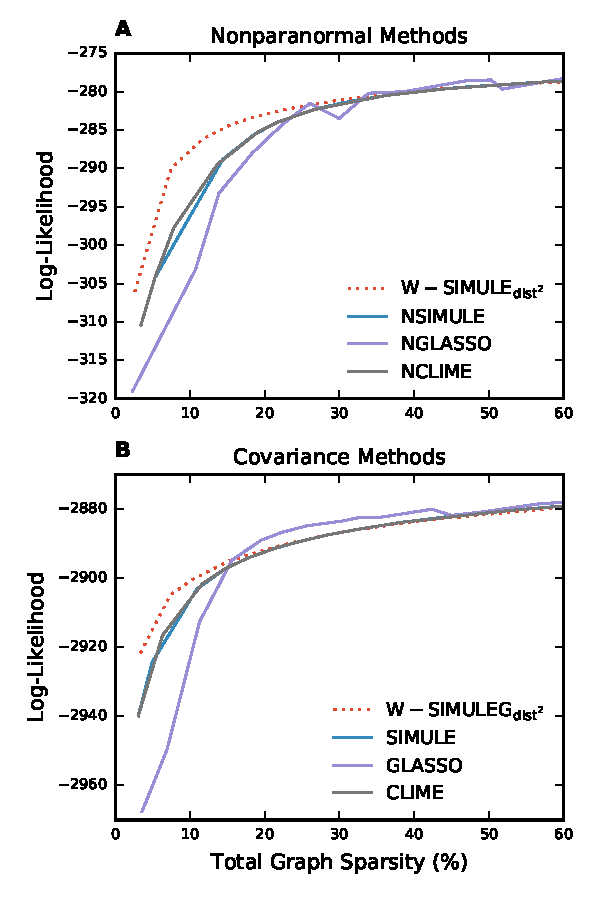
\includegraphics[width=\columnwidth]{../../plots/ll/ll_best.pdf}
	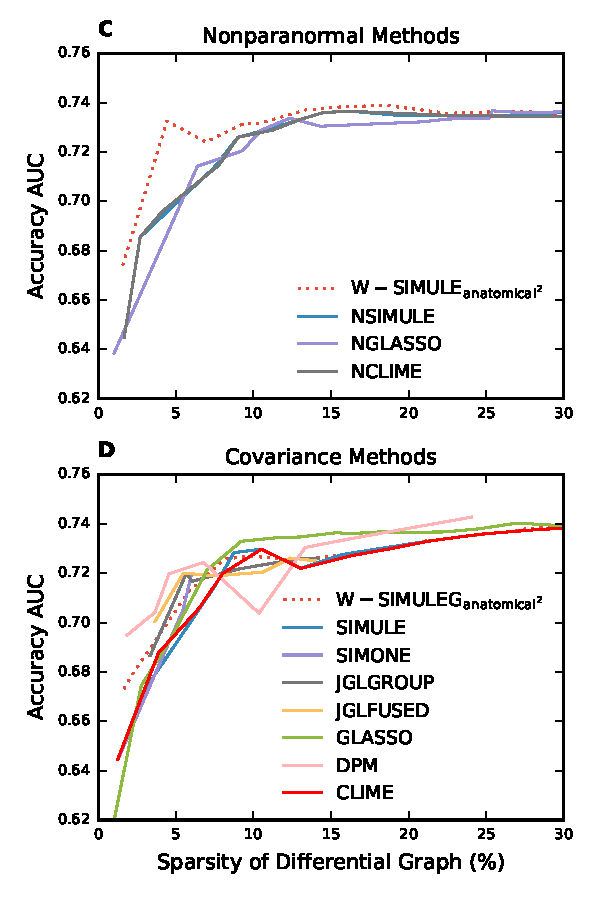
\includegraphics[width=\columnwidth]{../../plots/acc/['full_1']_best_ridge_au_auc.pdf}
	\caption{Model performace measured by log-likelihood and classification accuracy. A and B show the log-likelihood versus number edges included in the model. Note that A and B are not directly comparable, as A takes as input the Kendall correlation matrix while B uses the sample covariance matrix. Simone is not shown as it yields a log-likelihood below --$10^{-6}$ and JGL is omitted because it fails to converge when run on the entire dataset. C and D show the accuracy AUC versus number of edges included in the model. Edges represent features that were fed into a binary ridge regression classifier. C shows the edges using nonparanormal methods while D shows the edges using covariance methods. The same process was carried out using elastic net and lasso regression, but these classifiers perform more poorly than ridge regression.}
	\label{fig:performance}
\end{figure*}

Additionally, the study aims to use classification scores to compare how well multiple sparse graphical model algorithms are able to select edges that are most representative of the dataset. Several recent studies perform classification on the dataset with varying accuracies (summarized in  Table~\ref{background_table}). Notably, few studies classify all of these subjects in the ABIDE dataset. In fact, no study achieving over 63\% classification accuracy uses more than 700 subjects.

Classification is performed using 3-fold cross validation. The data is randomly partitioned into 3 equal sets: a training set, a validate set, and a test set. The graphical model produces graphs for the autism group and the control group using the training set. Then, the difference graph is calculated by subtracting the autism graph from the control graph. Then, the nonzero edges in the difference graph are used for feature selection; namely, for every edge between ROI x and ROI y, the mean value of x$\cdot$y over time was selected as a feature. These features are fed to a general linear ridge regressor (ridge regression outperformed lasso and elastic net regression). This method evaluates the learned structure of the graphs; in all cases, self-edges are disallowed. The regressor is trained via cross-validation using only the validate set. Finally, accuracy for the classifier is reported on the test set. This full process is performed and averaged over 3 folds for each graphical model examined here. 

The resulting accuracy AUC for each level of sparsity is shown in Figure~\ref{fig:performance} C,D. The new model outperforms all baselines, particularly at low sparsities which are most biophysically plausible. 

\subsection{Parameter Searching}

\begin{table*}[ht]
	\caption{Variations of prior and epsilon. All methods are nonparanormal.}
	\label{tab:parameter_searching}
	\vskip 0.15in
	\begin{center}
		\begin{small}
			\begin{sc}
				\begin{tabular}{lcccc}
				    \multicolumn{5}{c}{\textbf{Changing Prior ($\mathbf{\epsilon = 1}$)}}\\
					\abovespace\belowspace
					Prior Name & \scell[]{Log-Likelihood AUC\\(Sparsity $\leq$ 7\%)} & \scell[]{Accuracy AUC\\(Sparsity $\leq$ 7\%)} & \scell[]{Log-Likelihood AUC\\(Sparsity $\leq$ 15\%)} & \scell[]{Accuracy AUC\\(Sparsity $\leq$ 15\%)}\\
					\hline
					\abovespace
Distance & -261.91 & 0.68 & -266.84 & 0.70 \\
$\text{Distance}^2$ & -262.32 & 0.65 & -249.93 & 0.68 \\
Anatomical1 & -102.10 & 0.68 & -269.54 & 0.72 \\
Anatomical2 & -119.54 & 0.68 & -267.53 & 0.72 \\
					\hline\\
					\multicolumn{5}{c}{\textbf{Changing $\epsilon$ (Prior = Anatomical2)}}\\
					\abovespace\belowspace
					Epsilon & \scell[]{Log-Likelihood AUC\\(Sparsity $\leq$ 7\%)} & \scell[]{Accuracy AUC\\(Sparsity $\leq$ 7\%)} & \scell[]{Log-Likelihood AUC\\(Sparsity $\leq$ 15\%)} & \scell[]{Accuracy AUC\\(Sparsity $\leq$ 15\%)}\\
					\hline
					\abovespace
0.5 & -128.84 & 0.70 & -296.49 & 0.57 \\
0.1 & -134.12 & 0.62 & -235.93 & 0.70 \\
$10^{-6}$ & -136.34 & 0.63 & -240.15 & 0.69 \\
					\hline
				\end{tabular}
			\end{sc}
		\end{small}
	\end{center}
	\vskip -0.1in
\end{table*}
\FloatBarrier

 Figure~\ref{fig:edge_lengths} shows the effectiveness of the distance prior at reducing average edge length. 
 
\subsection{Connectome}
The new model yields connectomes at varying levels of sparsity. One such overall connectome, generated from the entire dataset, is shown in Figure~\ref{fig:connectome}.

\begin{figure}[H]
	\centering
	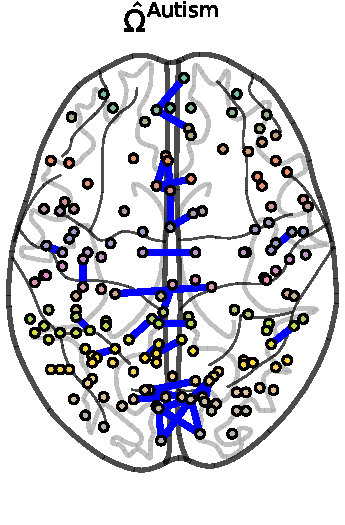
\includegraphics[width=\columnwidth]{../../plots/connectomes/autism.pdf}
	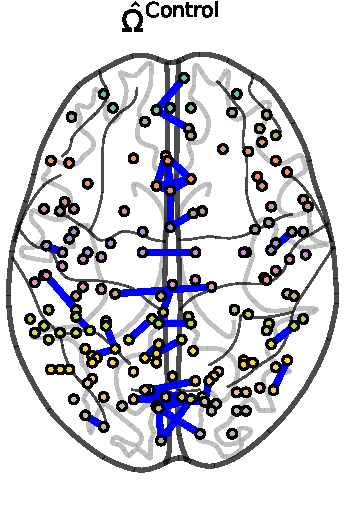
\includegraphics[width=\columnwidth]{../../plots/connectomes/control.pdf}
	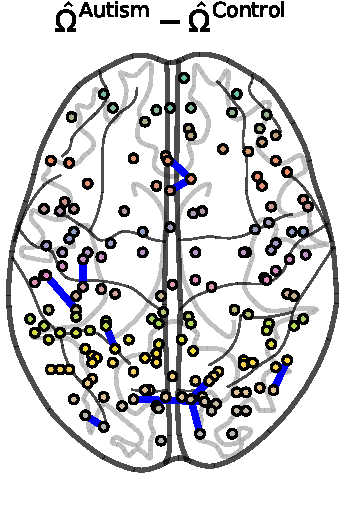
\includegraphics[width=\columnwidth]{../../plots/connectomes/diff.pdf}
	\caption{Example connectome generated by NWELM. The context-specific graphs for the autism, control, and their difference (e.g. control subtracted from autism) are shown. Visualization performed with nilearn \cite{abraham2014machine}.}
	\label{fig:connectome}
\end{figure}

\FloatBarrier
\section{Conclusions}
\label{conclusions}

WELM effectively enforces a prior while imposing sparsity and taking advantage of multi-task learning. The connectomes generated here demonstrate the expected connectivity within anatomic regions, as expected. They also selectively highlight the connections that are important for distinguishing between autism and control gorups; this can help researchers in neuroscience to pinpoint the neural connectivity basis of autism. This model's application to neuroscience is very important and it can be readily applied to several other functional connectivity datasets \cite{milham2012adhd,smith2013resting}. As datasets become more complex and include more structural (e.g. MRI data) coupled with functional (e.g. fMRI data), this model will become increasingly important. Studies with small sample sizes, such as task-specific studies require strong priors in order to reasonably compute connectivity \cite{real2017neural}.

Additionally, as the spatial resolution of fMRI increases, spatial penalization will become more imporant to construct increasingly accurate ROIs and brain connections. Determining how to construct these ROIs is an active area of research \cite{craddock2015connectomics,thirion2014fmri}, and using different groupings as input to this model can help to evaluate them.

% Acknowledgements should only appear in the accepted version. 
%\section*{Acknowledgements}

\bibliography{refs_abide}
\bibliographystyle{icml2017}

\section*{Supplement}
\setcounter{figure}{0}
\renewcommand{\thefigure}{S\arabic{figure}}
\setcounter{table}{0}
\renewcommand{\thetable}{S\arabic{table}}

\begin{table*}[ht]
	\caption{Classification accuracy obtained on ABIDE dataset by previous studies. In general, there is a significant classification improvement over randomness (50\%). Many of these studies employ different preprocessing, training, and validation schemes. Smaller subsets of the data are generally able to achieve better performance, as correlations can be found in these small datasets that can overestimate the accuracy of a classifier \cite{haar2014anatomical}.}
	\label{background_table}
	\vskip 0.15in
	\begin{center}
		\begin{small}
			\begin{sc}
				\scriptsize
				\begin{tabulary}{\textwidth}{CCCCCCCCCC}
					\hline
					\abovespace\belowspace
					Study & \textbf{This Study} & \citet{ghiassian2013learning} & \citet{nielsen2013multisite}& \citet{haar2014anatomical} & \citet{iidaka2015resting}& \citet{haar2014anatomical} & \citet{chen2015diagnostic} & \citet{chen2016multivariate} & \citet{plitt2015functional}\\
					\hline
					%\abovespace
					Total Subjects & 871 & 1111 & 964  & 906 & 640 & 590& 252 & 240 & 178 \\ \hline
					Autism Subjects & 403 & 538 & 447  & 453 & 328 & 295& 126 & 112 & 89 \\ \hline
					Control Subjects  & 468 & 573 & 517& 453 & 312 & 295 & 126 & 128 & 89 \\ \hline
					Method & See Model & MRMR selection of HOG features & GLM &  LDA and QDA & Probabilistic neural network & LDA and QDA & Random forest & S	VMs with slow frequency range & L2LR \\ \hline
					\belowspace
					Accuracy (\%) & \textbf{X} & 63 & 60 & $\sim$50 & 90& 60 & 91 & 79 & 71 \\ 
					\hline
				\end{tabulary}
			\end{sc}
		\end{small}
	\end{center}
	\vskip -0.1in
\end{table*}
\FloatBarrier
\begin{figure}[H]
	\centering
	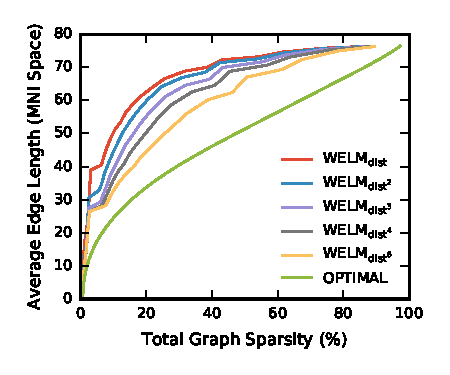
\includegraphics[width=\columnwidth]{../../plots/edge_stats/edge_stats_v_num_features.pdf}
	\caption{WELM effectively enforces the prior. Average edge-length, as a function of the number of edges for different models decreases as the spread between the prior weights increases. ``Optimal" line shows the lowest possible average edge length for different numbers of edges.}
	\label{fig:edge_lengths}
\end{figure}

\begin{table}[H]
	\caption{Range of parameters generating the graphs shown in the Experiments section.}
	\label{tab:params}
	\vskip 0.15in
	\begin{center}
		\begin{small}
			\begin{sc}
				\begin{tabular}{lcc}
					\hline
					\abovespace\belowspace
					Method & $\lambda_1$ & $\lambda_2$ \\
					\hline
					\abovespace
					CLIME & [0.1,0.5] & \\
					GLASSO & [0.1,0.5] & \\
					JGL & [0.1,0.5] & [0.4,0.5]\\
					DPM & [0.1,0.5] & \\
					SIMONE & [0.1,0.5] & \\
					WEIGHTED SIMULE & [0.1,0.5] & [0.4,0.5]\\
					\belowspace
					SIMULE & [0.1,0.5] & [0.4,0.5]\\
					\hline
				\end{tabular}
			\end{sc}
		\end{small}
	\end{center}
	\vskip -0.1in
\end{table}

\end{document} 